\documentclass{./../../Latex/teaching_slides}
\begin{document}

\title{ECON 441 \\ \vspace{0.4em} \normalsize Introduction to Mathematical Economics}
\author{Div Bhagia}
\date{Lecture 2: Linear Algebra}

%%%%%%%%%%%%%%%%%%%%
\begin{frame}[noframenumbering, plain]
\maketitle
\end{frame}

%%%%%%%%%%%%%%%%%%%%
\begin{frame}{A Simple Economic Model}
$ q $: quantity of hats, $p$: price of a single hat \\~\\
Demand for hats: $ q = 100-2p $ \\ \vspace{0.2em}
\begin{center}
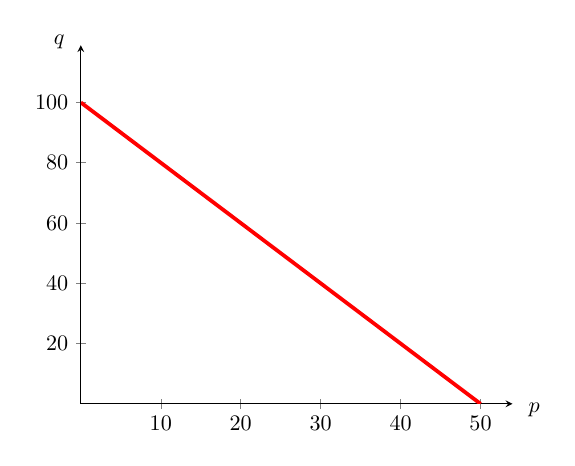
\begin{tikzpicture}[scale=0.8]
\begin{axis}[axis lines = center, xlabel = \(p\), ylabel = \(q\), ytick distance=20, xtick distance=10, ymax=119, xmax = 54, xlabel style={at={(axis description cs:1.05,0.025)}, anchor=north}, ylabel style={at={(axis description cs:-0.05,1.05)}, anchor=north}]
\addplot [domain=0:50, samples=100, color=red, line width = 0.6mm]{100-2*x};
\end{axis}
\end{tikzpicture}
\end{center}
\end{frame}

%%%%%%%%%%%%%%%%%%%%
\begin{frame}{A Simple Economic Model}
$ q $: quantity of hats, $p$: price of a single hat \\~\\
Supply for hats: $ q = 20+3p $ \\ \vspace{0.2em}
\begin{center}
\begin{tikzpicture}[scale=0.8]
\begin{axis}[axis lines = center, xlabel = \(p\), ylabel = \(q\), ytick distance=20, xtick distance=10, ymax=119, xmax = 54, xlabel style={at={(axis description cs:1.05,0.025)}, anchor=north}, ylabel style={at={(axis description cs:-0.05,1.05)}, anchor=north}]
\addplot [domain=0:50, samples=100, color=black, line width = 0.6mm]{20+3*x};
\end{axis}
\end{tikzpicture}
\end{center}
\end{frame}

%%%%%%%%%%%%%%%%%%%%
\begin{frame}{A Simple Economic Model}
$ q $: quantity of hats, $p$: price of a single hat \\~\\
Demand for hats:
$$ q = 100-2p $$
Supply for hats:
$$ q = 20+3p $$ \\~\\
\textit{Equilibrium}: At what price will both demand and supply be equal? 
\end{frame}

%%%%%%%%%%%%%%%%%%%%
\begin{frame}{Equilibrium}
\textit{Equilibrium}: At what price will both demand and supply be equal? 
$$ 100-2p = 20+3p \rightarrow  p^* = \$16  $$ \\~\\
\pause
What is the quantity traded at this price? 
$$ q ^* = 100-2 \times 16 = 20+3 \times 16 = 68  $$ \\~\\
$q ^*$ and $p^*$ are determined simultaneously. 
\end{frame}

%%%%%%%%%%%%%%%%%%%%
\begin{frame}{Equilibrium}
\begin{center}
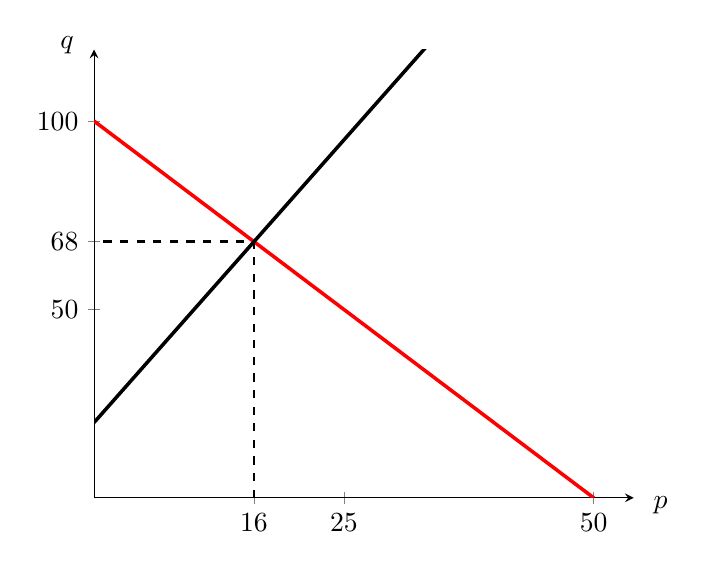
\begin{tikzpicture}
\begin{axis}[axis lines = center, xlabel = \(p\), ylabel = \(q\), ytick distance=50, xtick distance=25, ymax=119, xmax = 54, xlabel style={at={(axis description cs:1.05,0.025)}, anchor=north}, ylabel style={at={(axis description cs:-0.05,1.05)}, anchor=north}, extra x ticks ={16}, extra y ticks ={68}]
\addplot [domain=0:50, samples=100, color=red, line width = 0.45mm]{100-2*x};
\addplot [domain=0:50, samples=100, color=black, line width = 0.45mm]{20+3*x};
\draw [dashed, line width = 0.35mm] (axis cs:16,0) -- (axis cs:16,68) -- (axis cs:0,68);
\end{axis}
\end{tikzpicture}
\end{center}
\end{frame}


%%%%%%%%%%%%%%%%%%%%
\begin{frame}{Matrix Algebra}
We solved a \textit{system} of two (linear) equations in two variables. \\~\\
Complex economic models: multiple equations with multiple variables \\~\\
Hard to just wing it... Enter, Matrix Algebra! \\~\\
Matrix Algebra can help us write complex system of equations compactly and solve them
\end{frame}

%%%%%%%%%%%%%%%%%%%%
\begin{frame}{A Simple Economic Model}
$ q $: quantity of hats, $p$: price of a single hat \\~\\
Demand for hats: $ q = 100-2p $ \\~\\
Supply for hats: $ q = 20+3p $ \\~\\
Rewrite the two equations: 
\begin{align*}
q + 2p &= 100 \\ q-3p &= 20
\end{align*}
\end{frame}

%%%%%%%%%%%%%%%%%%%%
\begin{frame}{A Simple Economic Model}
Two equations in two unknowns:
\begin{align*}
q + 2p &= 100 \\ q-3p &= 20
\end{align*}
Can write this as:
$$ Ax = b $$
where
$$A = \begin{bmatrix}
1 & 2 \\
1 & -3 
\end{bmatrix} \quad 
x = \begin{bmatrix}
q \\
p 
\end{bmatrix} \quad 
b = \begin{bmatrix}
100 \\
20 
\end{bmatrix}$$ \\~\\
These arrays are called matrices. 
\end{frame}


%%%%%%%%%%%%%%%%%%%%
\begin{frame}{Today}
\begin{witemize}
\item Matrices: Addition, Subtraction, and Scalar Multiplication
\item Matrix Multiplication
\item Vectors
\item Identity and Null Matrices 
\item Transpose and Inverse of a Matrix \\~\\
\end{witemize}
Textbook reference: 4.1-4.6
\end{frame}

%\section{Matrices}
%%%%%%%%%%%%%%%%%%%%
\begin{frame}{Matrices}
A \textit{matrix} is a rectangular array of numbers, parameters, or vectors. \\~\\
Example. $A = \begin{bmatrix}
2 & 3 & 1 \\
-1 &4 & 6
\end{bmatrix}$ 
\vspace{2em} \\
Dimensions of matrix:
\begin{itemize}
\item Number of rows ($m$)
\item Number of columns ($n$)
\end{itemize}
\end{frame}

%%%%%%%%%%%%%%%%%%%%
\begin{frame}{Matrices}
A matrix with $m$ rows and $n$ columns is referred to as an $m \times n$ matrix \\~\\
What's the dimension of $A$? \\~\\
 $$A = \begin{bmatrix}
2 & 3 & 1 \\
-1 &4 & 6
\end{bmatrix}_{\pause 2 \times 3}$$ \\~\\
\end{frame}

%%%%%%%%%%%%%%%%%%%%
\begin{frame}{Matrices}
$$A = \begin{bmatrix}
a_{11} & a_{12} & a_{13} & \hdots & a_{1n} \\
a_{21} & a_{22} & a_{23} & \hdots & a_{2n} \\
\vdots & \vdots & \vdots & \vdots & \vdots \\
a_{m1} & a_{m2} & a_{m3} & \hdots & a_{mn} \\
\end{bmatrix}$$

\vspace{2em}
Can write it more compactly
$$ A = [ a_{ij} ] \quad i=1,2,...,m; j=1,2,...,n$$
\end{frame}

%%%%%%%%%%%%%%%%%%%%
\begin{frame}{Matrices}
\textit{Square matrix}: equal number of rows and columns \\~\\
Example.
$$A = \begin{bmatrix}
a_{11} & a_{12} & a_{13} \\
a_{21} & a_{22} & a_{23} \\
a_{31} & a_{32} & a_{33} \\
\end{bmatrix}_{3\times 3}$$
\end{frame}

%%%%%%%%%%%%%%%%%%%%
\begin{frame}{Matrices}
Two matrices are \textit{equal} if all their elements are identical. \\~\\
Example.
$$A = \begin{bmatrix}
1 & 8  \\
4 &-1  \\
\end{bmatrix} \neq
 \begin{bmatrix}
1 & 8  \\
4 & 2  \\
\end{bmatrix}$$

\vspace{2em}
So $A=B$ if and only if $a_{ij} = b_{ij}$ for all $i, j$
\end{frame}

%%%%%%%%%%%%%%%%%%%%
\begin{frame}{Matrix Addition and Subtraction}
\begin{witemize}
\item How to add or take the difference between two matrices? 
\item[] \hspace{1em} $\rightarrow$ Element-by-element
\item[] \hspace{1em} $\rightarrow$  Matrices have to have same dimension \\~\\
\end{witemize}
Example.
$$A = \begin{bmatrix}
2 & 3 \\
4 & -6 
 \end{bmatrix} \quad \quad
B = \begin{bmatrix}
1 & 8 \\
-2 & 3
\end{bmatrix}$$
\begin{witemize}
\item What is $A+B$ and $A-B$?
\end{witemize}
\end{frame}

%%%%%%%%%%%%%%%%%%%%
\begin{frame}{Scalar Multiplication}
How to multiply a scalar to a matrix? 
$$ \lambda \begin{bmatrix} a_{11} & a_{12} & a_{13} \\ 
a_{21} & a_{22} & a_{23} \\  \end{bmatrix} = \begin{bmatrix} \lambda a_{11} & \lambda a_{12} & \lambda a_{13} \\ 
\lambda a_{21} & \lambda a_{22} & \lambda a_{23} \\  \end{bmatrix} $$
Example.
$$A = \begin{bmatrix}
2 & 3 \\
4 & -6 
\end{bmatrix}  \quad \quad
B = \begin{bmatrix}
1 & 8 \\
-2 & 3
\end{bmatrix}$$
What is $2B$ and $A-2B$?
\end{frame}

%%%%%%%%%%%%%%%%%%%%
\begin{frame}{Matrix Multiplication}
A whole new animal... \\~\\

Only possible to multiply two matrices, $A_{m \times n}$ and $B_{p \times q}$ to get $AB$ if $ n = p $ i.e.
$$\text{number of columns in } A = \text{ number of rows in } B $$ 
\\~\\

Example.
$A = \begin{bmatrix}
2 & 3 & 1 \\
4 & -6 & -2
\end{bmatrix}_{2 \times 3}$ 
$B = \begin{bmatrix}
1 & 8 \\
-2 & 3
\end{bmatrix}_{2 \times 2}$ \\~\\

Cannot do $AB$, but can do $BA$
\end{frame}

%%%%%%%%%%%%%%%%%%%%
\begin{frame}{Matrix Multiplication}
Another example.
$$A = \begin{bmatrix}
2 & 3 & 1 \\
4 & -6 & -2
\end{bmatrix}_{2 \times 3}
B = \begin{bmatrix}
1 \\
-2 \\
4
\end{bmatrix}_{3 \times 1}$$ \\
Can we multiply $A$ and $B$ to find $C=AB$? \\~\\
\pause Yes, since $A$ has 3 rows which is equal to the number of columns in $B$. \\~\\
Also, the dimension of $C$ will be $2 \times 1$.
\end{frame}



%%%%%%%%%%%%%%%%%%%%
\begin{frame}{Matrix Multiplication}
So how to actually multiply these matrices? \\~\\
$$ C = AB$$
$$ c_{ij} = a_{i1} b_{1j} + a_{i2} b_{2j} + ... + a_{in} b_{nj} = \sum_{k=1}^n a_{ik} b_{kj}   $$

\vspace{1em}
The \alert{element $c_{ij}$} is obtained by multiplying term-by-term the entries of the \alert{$i$th row of $A$} and \alert{$j$th column of $B$}. 
\end{frame}


%%%%%%%%%%%%%%%%%%%%
\begin{frame}{Matrix Multiplication: Examples}
$$A = \begin{bmatrix}
a_{11} & a_{12} &  a_{13} \\
a_{21} & a_{22} &  a_{23} \\
\end{bmatrix}_{2 \times 3}
B = \begin{bmatrix}
b_{11} & b_{12} \\
b_{21} & b_{22} \\
b_{31} & b_{32} \\
\end{bmatrix}_{3 \times 2}$$ \\
Here, \small
$$C = AB = \begin{bmatrix}
 a_{11}b_{11} +  a_{12}b_{21} + a_{13}b_{31} &  a_{11}b_{12} +  a_{12}b_{22} + a_{13}b_{32} \\
  a_{21}b_{11} +  a_{22}b_{21} + a_{23}b_{31} &  a_{21}b_{12} +  a_{22}b_{22} + a_{23}b_{32} \\
\end{bmatrix}_{2 \times 2} $$
\end{frame}


%%%%%%%%%%%%%%%%%%%%
\begin{frame}{Matrix Multiplication: Examples}
$$A = \begin{bmatrix}
2 & 3 & 1 \\
4 & -6 & -2
\end{bmatrix}_{2 \times 3}
B = \begin{bmatrix}
1 \\
-2 \\
4
\end{bmatrix}_{3 \times 1}$$ 
\\~\\
\pause
$$C = AB =  \begin{bmatrix}
2 \times 1 + 3 \times -2 + 1 \times 4  \\
4 \times 1 + -6 \times -2 + -2 \times 4  \\
\end{bmatrix}_{2 \times 1} = 
\begin{bmatrix}
0  \\
8  \\
\end{bmatrix}_{2 \times 1} \vspace{1cm}$$
\end{frame}

%%%%%%%%%%%%%%%%%%%%
\begin{frame}{Matrix Multiplication: Examples}
$$A = \begin{bmatrix}
1 & 3  \\
2 & 8 \\
4 & 0 \\
\end{bmatrix} \quad
B = \begin{bmatrix}
5 \\
9 \\
\end{bmatrix}$$ 
\end{frame}

%%%%%%%%%%%%%%%%%%%%
\begin{frame}{A Simple Economic Model}
$$A = \begin{bmatrix}
1 & 2 \\
1 & -3 
\end{bmatrix} \quad 
x = \begin{bmatrix}
q \\
p 
\end{bmatrix} \quad 
b = \begin{bmatrix}
100 \\
20 
\end{bmatrix}$$
\\~\\

What is $Ax$? 
\pause
$$Ax = \begin{bmatrix}
q + 2p\\
q-3p
\end{bmatrix}$$
\vspace{1em}
\pause

Setting $Ax=b$ gives us back our demand and supply equations. 
\end{frame}

%%%%%%%%%%%%%%%%%%%%
\begin{frame}{}
\centering

\includegraphics[scale=0.3]{AI_linal.jpeg}
\end{frame}

%\section{Vectors}
%%%%%%%%%%%%%%%%%%%%
\begin{frame}{Vectors}
\begin{witemize}
\item Matrices with only one column: column vectors 
$$ x =  \begin{bmatrix}
x_1\\
x_2 \\
\vdots \\
x_n
\end{bmatrix} $$
\item Matrices with only one row: row vectors
$$ x' =  \begin{bmatrix}
x_1 &
x_2 & \hdots &
x_n
\end{bmatrix} $$
\end{witemize}
\end{frame}

%%%%%%%%%%%%%%%%%%%%
\begin{frame}{Inner Product}
Inner product of two vectors each with $n$ elements:
$$ u \cdot v = u_1 v_1 + u_2 v_2 +...+ u_n v_n = \sum_{i=1}^n u_i v_i $$ 
Example. $$u = \begin{bmatrix} 1 \\ 5 \\ 2 \end{bmatrix} \quad \quad v = \begin{bmatrix} 2 \\ 1 \\ 3 \end{bmatrix}$$
\end{frame}

%%%%%%%%%%%%%%%%%%%%
\begin{frame}{Linear Dependence}
A set of vectors is said to be \textit{linearly dependent} if and only if any one of them can be expressed as a linear combination of the remaining vectors. \\~\\
Example.$$ v_1 =  \begin{bmatrix}
1\\
2 \\
\end{bmatrix} \quad \quad v_2 = \begin{bmatrix}
2\\
4 \\
\end{bmatrix}$$
\end{frame}

%%%%%%%%%%%%%%%%%%%%
\begin{frame}{Linear Dependence}
A set of vectors is said to be \textit{linearly dependent} if and only if any one of them can be expressed as a linear combination of the remaining vectors. \\~\\
Example.$$ v_1 =  \begin{bmatrix}
3\\
2 \\
\end{bmatrix} \quad \quad v_2 = \begin{bmatrix}
1\\
3 \\
\end{bmatrix} \quad \quad v_3 = \begin{bmatrix}
1\\
-4 \\
\end{bmatrix} $$
\end{frame}

%%%%%%%%%%%%%%%%%%%%
\begin{frame}{Linear Dependence}
A set of $m$-vectors $v_1, v_2, ...,v_n$ is linearly dependent if and only if there exists a set of scaler $k_1, k_2, ..., k_n$ (not all zero) such that:
$$ \sum_{i=1}^n k_i v_i = 0 \quad (m \times 1) $$
\end{frame}

%\section{Identity and Null Matrices}
%%%%%%%%%%%%%%%%%%%%
\begin{frame}{Identity Matrices}
Square matrix with $1$s in its \textit{principal diagonal} and $0$s elsewhere \\~\\
A $2 \times 2$ identity matrix:
$$ I_2 = \begin{bmatrix}
1 & 0\\
0 & 1 \\
\end{bmatrix}$$
A $3 \times 3$ identity matrix:
$$ I_3 = \begin{bmatrix}
1 & 0 & 0 \\
0 & 1 & 0\\
0 & 0 & 1
\end{bmatrix}$$

\end{frame}

%%%%%%%%%%%%%%%%%%%%
\begin{frame}{Identity Matrices}
Acts like 1, 
$$ AI = IA = A $$

\vspace{2em}

Example. 
$$A = \begin{bmatrix}
2 & 3 & 1 \\
4 & -6 & 2
\end{bmatrix}$$
\end{frame}

%%%%%%%%%%%%%%%%%%%%
\begin{frame}{Idempotent Matrices}
A matrix is an \textit{idempotent} matrix if it remains unchanged when multiplied by itself any number of times. \\~\\
$A$ is idempotent if and only if $A = A^k$. \\~\\
Is an identity matrix idempotent?
\end{frame}

%%%%%%%%%%%%%%%%%%%%
\begin{frame}{Null Matrix}
A null matrix is a matrix with all elements $0$. \\~\\
$$\begin{bmatrix}
0 & 0 & 0 \\
0 & 0 & 0
\end{bmatrix}$$
\begin{witemize}
\item $A + 0 = A$
\item $A 0 = 0$
\end{witemize}
\end{frame}

%%%%%%%%%%%%%%%%%%%%
\begin{frame}{Transpose of a Matrix}
Transpose of A: interchange rows and columns ($A'$) \\~\\
$$A = \begin{bmatrix}
2 & 3 & 1 \\
4 & -6 & 2
\end{bmatrix}$$
\end{frame}

%%%%%%%%%%%%%%%%%%%%
\begin{frame}{Transpose of a Matrix}
Transpose of A  ($A'$ or $A^T$): interchange rows and columns \\~\\
$$A = \begin{bmatrix}
2 & 3 & 1 \\
4 & -6 & 2
\end{bmatrix}$$
\end{frame}

%%%%%%%%%%%%%%%%%%%%
\begin{frame}{Transpose of a Matrix}
\begin{witemize}
\item A matrix $A$ is said to be \textit{symmetric} if $$A'=A$$
\item A matrix $A$ is said to be \textit{skew-symmetric} if $$A'=-A$$
\item A matrix $A$ is said to be \textit{orthogonal} if $$A'A=I$$
\end{witemize}
\end{frame}

%%%%%%%%%%%%%%%%%%%%
\begin{frame}{Example: Symmetric Matrix}
$$
A=\left[\begin{array}{rrr}
1 & 2 & 0 \\
2 & 3 & -5 \\
0 & -5 & 4
\end{array}\right]
$$
\end{frame}

%%%%%%%%%%%%%%%%%%%%
\begin{frame}{Example: Skew-symmetric Matrix}
$$
A=\left[\begin{array}{ccc}0 & -1 & 3 \\ 1 & 0 & -4 \\ -3 & 4 & 0\end{array}\right] 
$$
\end{frame}

%%%%%%%%%%%%%%%%%%%%
\begin{frame}{Example: Orthogonal Matrix}
$$
A=\left[\begin{array}{cc}
\frac{1}{\sqrt{2}} & -\frac{1}{\sqrt{2}} \\
\frac{1}{\sqrt{2}} & \frac{1}{\sqrt{2}}
\end{array}\right]
$$
\end{frame}

%%%%%%%%%%%%%%%%%%%%
\begin{frame}{Properties of Transposes}
$$
\begin{array}{l}
\left(A^{\prime}\right)^{\prime}=A \\~\\
(A+B)^{\prime}=A^{\prime}+B^{\prime} \\~\\
(A B)^{\prime}=B^{\prime} A^{\prime} \\~\\
\end{array}
$$
Example:
\( A=\left[\begin{array}{ll}4 & 1 \\ 9 & 0\end{array}\right] \quad B=\left[\begin{array}{ll}2 & 0 \\ 7 & 1\end{array}\right] \)
\end{frame}

%%%%%%%%%%%%%%%%%%%%
\begin{frame}{Inverse of a Matrix}
For a \textbf{square} matrix $A$, it's inverse $A^{-1}$ is defined as:
$$
A A^{-1}=A^{-1} A=I
$$

\vspace{2em}
 Squareness is a \textit{necessary} condition not a \textit{sufficient} condition \\~\\
 If a matrix's inverse exists, it's called a \textbf{nonsingular} matrix
\end{frame}

%%%%%%%%%%%%%%%%%%%%
%\begin{frame}{Inverse of a Matrix}
%If an inverse exists, it is unique. \\~\\
%Proof by contradiction. Let's say $B = A^{-1}$ and $C=A^{-1}$.
%Then, $$ AB=BA=I $$
% $$ AC=CA=I $$
%Pre-multiply both sides by $B$,
%$$ BAC=BCA=BI  \implies C=B $$
%\end{frame}

%%%%%%%%%%%%%%%%%%%%
\begin{frame}{Properties of Inverses}
$$ \left(A^{-1}\right)^{-1}=A $$ \\~\\
$$ (A B)^{-1}=B^{-1} A^{-1} $$ \\~\\
$$ \left(A^{\prime}\right)^{-1}=\left(A^{-1}\right)^{\prime} $$
\end{frame}

%%%%%%%%%%%%%%%%%%%%
\begin{frame}{Solution of Linear-Equation System}
$$ Ax = b $$
\pause

\vspace{1em}
Pre-multiply both sides by $A^{-1}$, 
$$ A^{-1} Ax = A^{-1} b \quad \implies x = A^{-1} b $$

\pause If $A$ is singular, a unique solution does not exist. 
\end{frame}

%%%%%%%%%%%%%%%%%%%%
\begin{frame}{Homework Problems}
  \begin{witemize}
  \normalsize
  \item Exercise 4.2: 1, 2, 4
  \item Exercise 4.4: 5 (e), 7
  \item Exercise 4.5: 1, 4 
  \item Exercise 4.6: 2, 6 \\~\\
\end{witemize}
Reminder: Quiz 1 is next week.
\end{frame}


\end{document}